\documentclass{article}
\usepackage[preprint]{neurips_2026}
\usepackage{graphicx}
\usepackage{hyperref}
\title{EvoChartCode: Evolution-Guided Chart Code Induction for Reliable Chart Reasoning}
\author{Anonymous}
\begin{document}
\maketitle
\begin{abstract}
Vision-language models remain brittle on chart question answering because perception, reasoning, formatting, and abstention are entangled in a single generation. EvoChartCode introduces explicit Chart Code as an intermediate representation, then uses question-conditioned selection, code-grounded reasoning, verification, and evolution to make chart reasoning inspectable. This report is generated only from completed local artifacts and marks incomplete full-scale jobs as incomplete rather than inferring results.
\end{abstract}
\section{Method}
EvoChartCode maps a chart image to validated Chart Code containing layout, axes, legends, colorbars, series, derived relations, uncertainty, and provenance. A selector exposes relevant evidence to a code-only or image-plus-code reasoner, and a verifier checks support before normalization.
\begin{figure}[h]\centering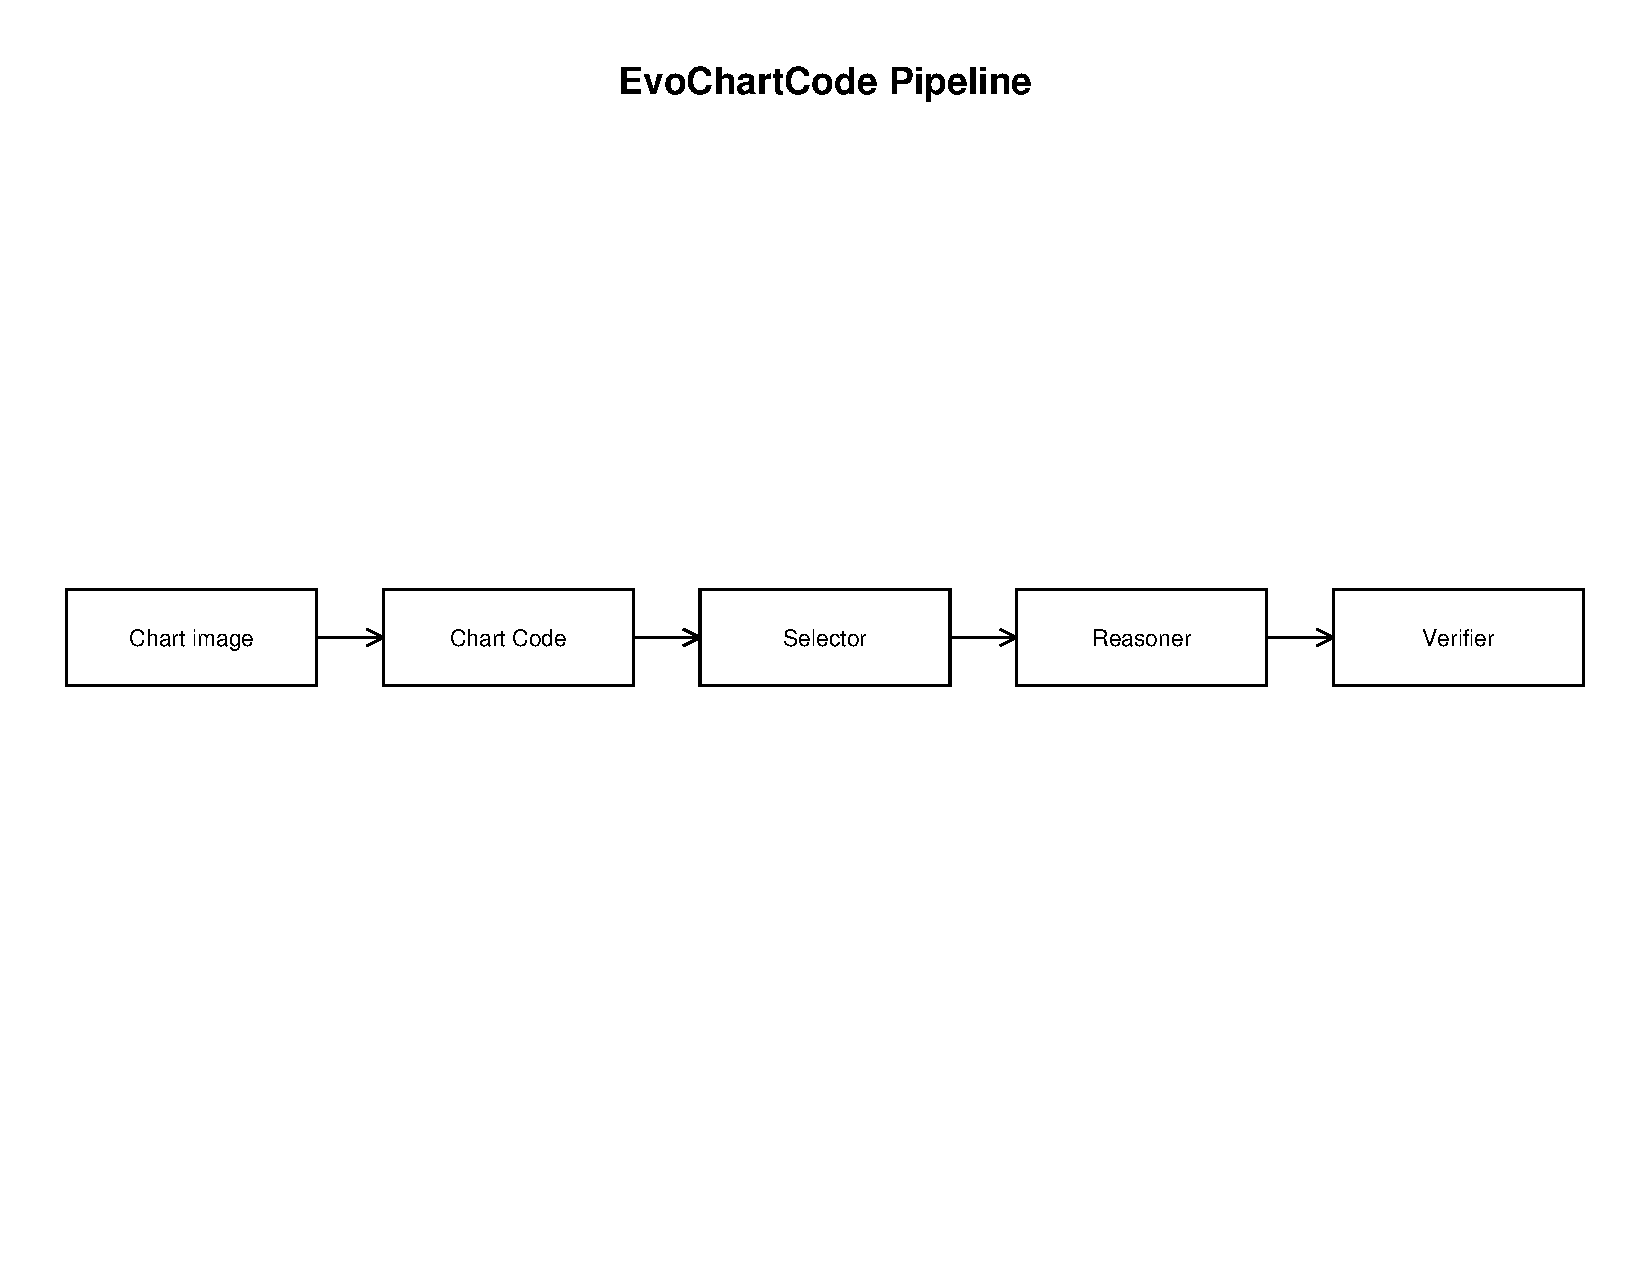
\includegraphics[width=0.95\linewidth]{figures/pipeline.pdf}\caption{EvoChartCode pipeline.}\end{figure}
\section{Main Results}
\begin{table}[h]\centering
\begin{tabular}{lrrrrr}
Method & N & EM & Relaxed & Invalid & Latency \\
\hline
Metadata/code-only & 128 & 0.2500 & 0.2812 & 0.0000 & 0.0006 \\
Qwen full EvoChartCode & 128 & 0.5312 & 0.5781 & 0.0000 & 13.2813 \\
\end{tabular}

\caption{CharXiv local validation results.}
\end{table}
\begin{table}[h]\centering
\begin{tabular}{lrrrr}
Backend & Charts & Quality & Axis evidence & Series/marks \\
\hline
Metadata & 300 & 0.5771 & 0.0000 & 0.0000 \\
Qwen & 32 & 0.8682 & 0.9375 & 0.9062 \\
\end{tabular}

\caption{Chart Code quality results.}
\end{table}
\section{Transfer}
\begin{table}[h]\centering
\begin{tabular}{llrrr}
Dataset & Status & N & EM & Relaxed \\
\hline
ChartQA & ready & 32 & 0.0000 & 0.0000 \\
PlotQA & ready & 32 & 0.0000 & 0.0000 \\
DVQA & ready & 32 & 0.0000 & 0.0000 \\
FigureQA & ready & 32 & 0.0000 & 0.0000 \\
\end{tabular}

\caption{Transfer results. Full Qwen metrics are used when completed; otherwise existing sample outputs are labeled by status.}
\end{table}
\section{Evolution}
\begin{figure}[h]\centering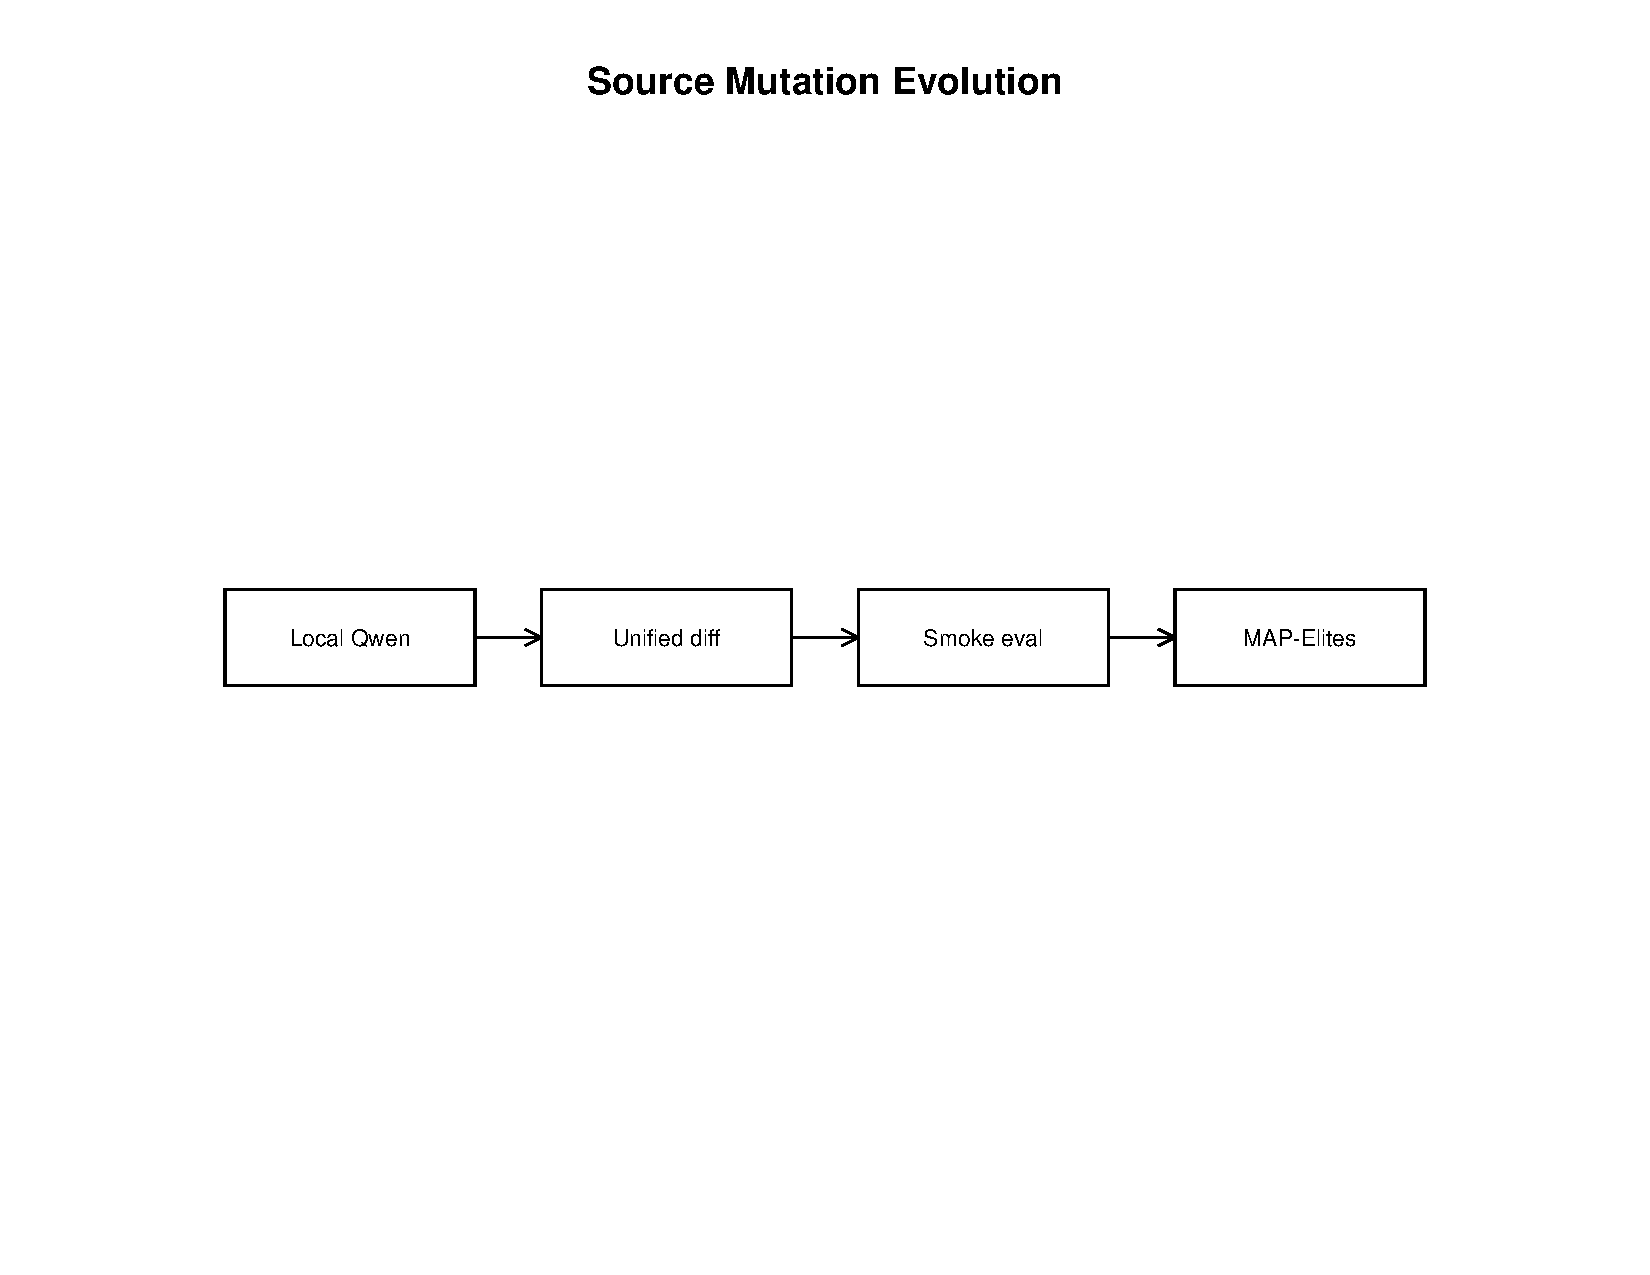
\includegraphics[width=0.95\linewidth]{figures/evolution.pdf}\caption{Local-Qwen source-code mutation loop.}\end{figure}
\section{Limitations}
Full benchmark-size transfer, multi-seed Qwen confidence intervals, and source-mutation evolution are checkpointed jobs. The paper should claim only completed measured results in the output JSON files.
\end{document}
